\documentclass[10pt]{article}
\usepackage[a4paper, total={18cm, 25cm}]{geometry}
\usepackage[hidelinks]{hyperref}
\usepackage{gensymb}
\usepackage{graphicx}
\usepackage{float}
\usepackage{tabularx}
\usepackage{wrapfig}
\usepackage{amssymb}
\usepackage{amsmath}
\numberwithin{equation}{subsection}
\usepackage{icomma}
\usepackage{booktabs}
\usepackage[utf8]{inputenc}
\usepackage[T1]{fontenc}
%\usepackage{arev}
\usepackage{newpxtext,newpxmath}

\title{The effects of exoplanet's shape on its transit light curve}
\author{Jiří Urbánek}

\begin{document}
\maketitle
I would like to thank the Faculty of Mathematics and Physics of Charles university for
making this project possible and especially Dr. Michaela Walterová for her amazing
guidance, willingness to help and tolerance of my faults.
\section{Introduction}
Several decades have passed since the discovery of the first exoplanet. To this day,
several thousand exoplanets have been confirmed and many more candidates are yet to
be confirmed. Transit photometry is the most common way of detecting these planets.
Transit photometry relies on the fact, that when a planet passes in front of its host
star, the star's brightness decreases. The relation between brightness and time can tell
us the ratio of the planet's and star's projected areas, the length of the orbit can tell
us their respetive masses and then we can calculate these parameters absolutely thanks to
the star's luminosity and spectrum.

Of course, planets aren't always strictly spherical and thus more variables come into play.
Namely, the planet can be ellipsoidal in shape with 3 distinct semi-axes. The aim of this
project was to determine the planet's transit light curve based on its shape.
\section{Methods}
\subsection{Angular size}
First, we need to determine how much the apparent size of the planet changes.
We can directly compare the difference between angular diameter of the planet at the 
point when it is closest to earth and at the point when it just crosses its host star,
and the difference between the angular diameter of two planets - one spherical and the
other ellipsoidal, both projecting to a circle and ellipse of the same respective area.
We can approximate the angular size as
\begin{equation}
  \delta = \frac{d}{D}
  \label{eq:angular-size}
\end{equation}
where $d$ is the diameter of the planet and $D$ is its distance to observer.
Let's assume that the planet orbits a circular orbit and that its distance from its
host star is $2\cdot10^8$ km. Next, we assume that the star is $10^{13}$ km far away
and its diameter is $10^5$ km. Let's be very generous and assume that the transit takes
place between $-\frac{\pi}{20}$ and $\frac{\pi}{20}$ radians from when the planet is
closest to the observer. Applying basic trigonometry, we get the equation
\begin{equation}
  D_2 = \sqrt{(D_1 + o)^2 + 1 -2 \cos(\sigma)(o^2 + D_1o)}
  \label{eq:D2}
\end{equation}
where $D_2$ is distance when the planet is the farthest away during its transit and $D_1$
is distance when the planet is the nearest, $o$ is the distance between the planet and
the star and $2\sigma$ is the angle of the whole transit. Calculating the difference
between the angular size for $D_1$ and $D_2$ with above mentioned values we get
$\Delta\delta = 2.02\cdot10^{-13}$.
This difference only becomes smaller for larger distances and smaller angles (we were very
generous in both cases), so we we will neglect all effects of angular size.
\subsection{Planet shape}
To some degree, all planets are non-spherical but the degree of oblateneness varies.
Oblateness depends on rotation, external gracitational tides and material rigidity. \cite{carter}
Close-in planets undergo strong tidal effects due to their parent star. Some of the 
concequences are that their spins and orbits change until equilibrium is reached, their
orbits become circular and synchronous and planetary bodies less spherical. \cite{correia1}
The shape of such a planet can generally be described by a 3-axis ellipsoid.
Such an ellipsoid, when projected to a plane, can be thought of as an ellipse with varying
semi-axes $a^{\prime}$ and $b^{\prime}$. Semi-axes $a^{\prime}$ and $b^{\prime}$ 
are described by the equation \cite{correia1} [thanks to Dr. Walterová]
\begin{equation}
  a^{\prime}, b^{\prime} = \frac{-\sqrt{-2(C^2 - 4AB)\left(A + B \mp\sqrt{(A -B)^2 + C^2}\right)}}{C^2 - 4AB}
  \label{eq:semi-axes}
\end{equation}
where 
\begin{equation}
  A = \frac{\sin^2\alpha}{a^2}+\frac{\cos^2\alpha}{b^2}, B = \frac{(\cos\alpha\cos i)^2}{a^2} + \frac{(\sin\alpha\cos i)^2}{b^2} + \frac{\sin^2 i}{c^2}, C = \left(\frac{1}{a^2} - \frac{1}{b^2}\right)\sin 2\alpha\cos i
  \label{eq:ABC}
\end{equation}
Parameters $a$, $b$ and $c$ are lengths of ellipsoid semi-axes such that $a$ and $b$
are on the plane of planet's orbit and $c$ is perpendicular. $\alpha$ is the phase of
the planet (in our case it is also the angle of the planet's orbit + some initial
phase). The inclination $i$ is 0 when the plane of orbit is perpendicular to line of sight
and $\frac{\pi}{2}$ when the planet passes directly across the centre of the star.
\subsection{Relative positions of a circle and an allipse, their overlap area}
Relative positions of an ellipse and a circle, can be described
in several parameters, namely the circle radius $r$ and centre $[h_1, k_1]$ and the
ellipse semi-axes $a$ and $b$, centre $[h_2, k_2]$ and angle $\phi$ against x-axis. For
our purposes, $\phi$ is described by equation \cite{correia1} [thanks to Dr. Walterová]
\begin{equation}
  \phi = \frac{1}{2}\arctan 2(-C, B-A)
  \label{eq:phi}
\end{equation}
There exist semi-analytical methods for calculating ellipse-ellipse intersection area
(analytical on a case-by-case basis) \cite{eeover} but in our case, due to higher
precision, we use a numerical method for calculating the overlap.
We calculate the relative positions on-the-fly by projecting the orbits of the planet
and the star to a plane tangent to the sky
\begin{equation}
  \begin{bmatrix}
    x_1 \\
    y_1 
  \end{bmatrix}
  = \frac{rm_2}{m_2+m_1}
  \begin{bmatrix}
    -\cos(\omega t) \\
    \cos(i)\cdot\sin(\omega t)
  \end{bmatrix},
  \begin{bmatrix}
    x_2 \\
    y_2 
  \end{bmatrix}
  = \frac{rm_1}{m_2+m_1}
  \begin{bmatrix}
    \cos(\omega t) \\
    -\cos(i)\cdot\sin(\omega t)
  \end{bmatrix}
  \label{eq:projected-orbit}
\end{equation}
where
\begin{equation}
  \omega = \frac{1}{r}\sqrt{G\frac{m_1 + m_2}{r}}
  \label{eq:omega}
\end{equation}
Here, $r$ is the distance between the star and the planet, $m_1$ and $m_2$ are the masses
of the star and the planet respectively, $i$ is the inclination of the orbit, $G$ is the
gravitational constant (in our case set to 1 for the sake of simplicity) and $t$ is the
time parameter.
\subsection{Realistic transit light curves}
Realistically, the transit light curve of a transiting planet isn't defined only by
the mass and shape of the star and the planet but depends on limb darkening of the star
and stellar activity too. Predicting stellar activity or accounting for limb darkening
is however beyond the scope of this project so we will only take mass and shape into
account.
\section{Results}
Now that we have all necessary equations, we can calculate the transit light curves.
In the following figures we will assume that the star is always the same size ($r_1 = 2$),
masses of the star and the planet remain the same ($m_1 = 8$, $m_2 = 1$), their relative
distance remains the same ($r = 10$) and $G$ is equal to 1. One orbit is signified by $t$.
For demonstration purposees, the parameters are very unrealistic.
\begin{figure}[H]
  \centering
  % GNUPLOT: LaTeX picture with Postscript
\begingroup
  \makeatletter
  \providecommand\color[2][]{%
    \GenericError{(gnuplot) \space\space\space\@spaces}{%
      Package color not loaded in conjunction with
      terminal option `colourtext'%
    }{See the gnuplot documentation for explanation.%
    }{Either use 'blacktext' in gnuplot or load the package
      color.sty in LaTeX.}%
    \renewcommand\color[2][]{}%
  }%
  \providecommand\includegraphics[2][]{%
    \GenericError{(gnuplot) \space\space\space\@spaces}{%
      Package graphicx or graphics not loaded%
    }{See the gnuplot documentation for explanation.%
    }{The gnuplot epslatex terminal needs graphicx.sty or graphics.sty.}%
    \renewcommand\includegraphics[2][]{}%
  }%
  \providecommand\rotatebox[2]{#2}%
  \@ifundefined{ifGPcolor}{%
    \newif\ifGPcolor
    \GPcolortrue
  }{}%
  \@ifundefined{ifGPblacktext}{%
    \newif\ifGPblacktext
    \GPblacktextfalse
  }{}%
  % define a \g@addto@macro without @ in the name:
  \let\gplgaddtomacro\g@addto@macro
  % define empty templates for all commands taking text:
  \gdef\gplbacktext{}%
  \gdef\gplfronttext{}%
  \makeatother
  \ifGPblacktext
    % no textcolor at all
    \def\colorrgb#1{}%
    \def\colorgray#1{}%
  \else
    % gray or color?
    \ifGPcolor
      \def\colorrgb#1{\color[rgb]{#1}}%
      \def\colorgray#1{\color[gray]{#1}}%
      \expandafter\def\csname LTw\endcsname{\color{white}}%
      \expandafter\def\csname LTb\endcsname{\color{black}}%
      \expandafter\def\csname LTa\endcsname{\color{black}}%
      \expandafter\def\csname LT0\endcsname{\color[rgb]{1,0,0}}%
      \expandafter\def\csname LT1\endcsname{\color[rgb]{0,1,0}}%
      \expandafter\def\csname LT2\endcsname{\color[rgb]{0,0,1}}%
      \expandafter\def\csname LT3\endcsname{\color[rgb]{1,0,1}}%
      \expandafter\def\csname LT4\endcsname{\color[rgb]{0,1,1}}%
      \expandafter\def\csname LT5\endcsname{\color[rgb]{1,1,0}}%
      \expandafter\def\csname LT6\endcsname{\color[rgb]{0,0,0}}%
      \expandafter\def\csname LT7\endcsname{\color[rgb]{1,0.3,0}}%
      \expandafter\def\csname LT8\endcsname{\color[rgb]{0.5,0.5,0.5}}%
    \else
      % gray
      \def\colorrgb#1{\color{black}}%
      \def\colorgray#1{\color[gray]{#1}}%
      \expandafter\def\csname LTw\endcsname{\color{white}}%
      \expandafter\def\csname LTb\endcsname{\color{black}}%
      \expandafter\def\csname LTa\endcsname{\color{black}}%
      \expandafter\def\csname LT0\endcsname{\color{black}}%
      \expandafter\def\csname LT1\endcsname{\color{black}}%
      \expandafter\def\csname LT2\endcsname{\color{black}}%
      \expandafter\def\csname LT3\endcsname{\color{black}}%
      \expandafter\def\csname LT4\endcsname{\color{black}}%
      \expandafter\def\csname LT5\endcsname{\color{black}}%
      \expandafter\def\csname LT6\endcsname{\color{black}}%
      \expandafter\def\csname LT7\endcsname{\color{black}}%
      \expandafter\def\csname LT8\endcsname{\color{black}}%
    \fi
  \fi
    \setlength{\unitlength}{0.0500bp}%
    \ifx\gptboxheight\undefined%
      \newlength{\gptboxheight}%
      \newlength{\gptboxwidth}%
      \newsavebox{\gptboxtext}%
    \fi%
    \setlength{\fboxrule}{0.5pt}%
    \setlength{\fboxsep}{1pt}%
    \definecolor{tbcol}{rgb}{1,1,1}%
\begin{picture}(7936.00,5102.00)%
    \gplgaddtomacro\gplbacktext{%
      \csname LTb\endcsname%%
      \put(946,704){\makebox(0,0)[r]{\strut{}$0.75$}}%
      \put(946,1539){\makebox(0,0)[r]{\strut{}$0.8$}}%
      \put(946,2375){\makebox(0,0)[r]{\strut{}$0.85$}}%
      \put(946,3210){\makebox(0,0)[r]{\strut{}$0.9$}}%
      \put(946,4046){\makebox(0,0)[r]{\strut{}$0.95$}}%
      \put(946,4881){\makebox(0,0)[r]{\strut{}$1$}}%
      \put(1078,484){\makebox(0,0){\strut{}$0$}}%
      \put(1724,484){\makebox(0,0){\strut{}$1000$}}%
      \put(2370,484){\makebox(0,0){\strut{}$2000$}}%
      \put(3016,484){\makebox(0,0){\strut{}$3000$}}%
      \put(3662,484){\makebox(0,0){\strut{}$4000$}}%
      \put(4309,484){\makebox(0,0){\strut{}$5000$}}%
      \put(4955,484){\makebox(0,0){\strut{}$6000$}}%
      \put(5601,484){\makebox(0,0){\strut{}$7000$}}%
      \put(6247,484){\makebox(0,0){\strut{}$8000$}}%
      \put(6893,484){\makebox(0,0){\strut{}$9000$}}%
      \put(7539,484){\makebox(0,0){\strut{}$10000$}}%
    }%
    \gplgaddtomacro\gplfronttext{%
      \csname LTb\endcsname%%
      \put(6552,1317){\makebox(0,0)[r]{\strut{}$i = 0.5 \pi$}}%
      \csname LTb\endcsname%%
      \put(6552,1097){\makebox(0,0)[r]{\strut{}$i = 0.47 \pi$}}%
      \csname LTb\endcsname%%
      \put(6552,877){\makebox(0,0)[r]{\strut{}$i = 0.45 \pi$}}%
      \csname LTb\endcsname%%
      \put(209,2792){\rotatebox{-270.00}{\makebox(0,0){\strut{}relative brightness}}}%
      \put(4308,154){\makebox(0,0){\strut{}time passed in terms of $\frac{1}{20000} t$}}%
    }%
    \gplbacktext
    \put(0,0){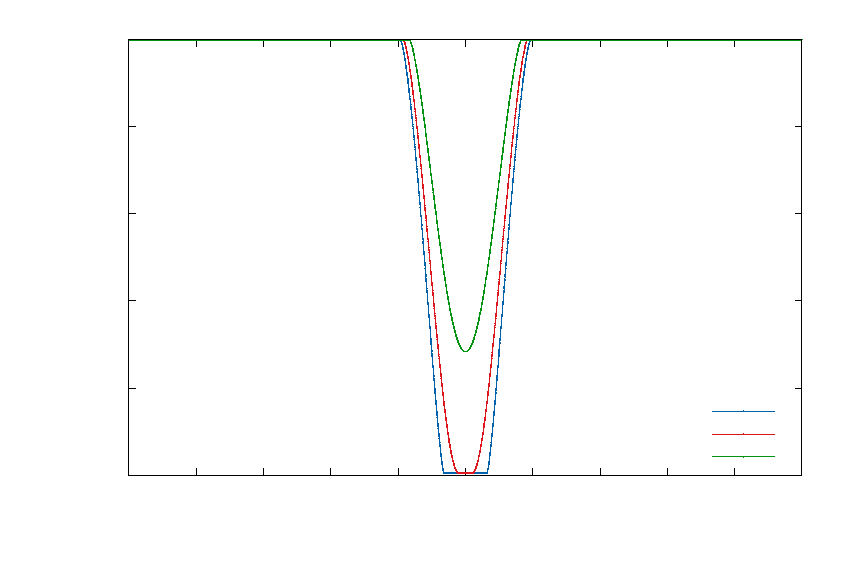
\includegraphics[width={396.80bp},height={255.10bp}]{figures/circles}}%
    \gplfronttext
  \end{picture}%
\endgroup

  \caption{Two spheres of the same size ($r_2$ = 1) but of different inclination $i$}
\end{figure}
\begin{figure}[H]
  \centering
  % GNUPLOT: LaTeX picture with Postscript
\begingroup
  \makeatletter
  \providecommand\color[2][]{%
    \GenericError{(gnuplot) \space\space\space\@spaces}{%
      Package color not loaded in conjunction with
      terminal option `colourtext'%
    }{See the gnuplot documentation for explanation.%
    }{Either use 'blacktext' in gnuplot or load the package
      color.sty in LaTeX.}%
    \renewcommand\color[2][]{}%
  }%
  \providecommand\includegraphics[2][]{%
    \GenericError{(gnuplot) \space\space\space\@spaces}{%
      Package graphicx or graphics not loaded%
    }{See the gnuplot documentation for explanation.%
    }{The gnuplot epslatex terminal needs graphicx.sty or graphics.sty.}%
    \renewcommand\includegraphics[2][]{}%
  }%
  \providecommand\rotatebox[2]{#2}%
  \@ifundefined{ifGPcolor}{%
    \newif\ifGPcolor
    \GPcolortrue
  }{}%
  \@ifundefined{ifGPblacktext}{%
    \newif\ifGPblacktext
    \GPblacktextfalse
  }{}%
  % define a \g@addto@macro without @ in the name:
  \let\gplgaddtomacro\g@addto@macro
  % define empty templates for all commands taking text:
  \gdef\gplbacktext{}%
  \gdef\gplfronttext{}%
  \makeatother
  \ifGPblacktext
    % no textcolor at all
    \def\colorrgb#1{}%
    \def\colorgray#1{}%
  \else
    % gray or color?
    \ifGPcolor
      \def\colorrgb#1{\color[rgb]{#1}}%
      \def\colorgray#1{\color[gray]{#1}}%
      \expandafter\def\csname LTw\endcsname{\color{white}}%
      \expandafter\def\csname LTb\endcsname{\color{black}}%
      \expandafter\def\csname LTa\endcsname{\color{black}}%
      \expandafter\def\csname LT0\endcsname{\color[rgb]{1,0,0}}%
      \expandafter\def\csname LT1\endcsname{\color[rgb]{0,1,0}}%
      \expandafter\def\csname LT2\endcsname{\color[rgb]{0,0,1}}%
      \expandafter\def\csname LT3\endcsname{\color[rgb]{1,0,1}}%
      \expandafter\def\csname LT4\endcsname{\color[rgb]{0,1,1}}%
      \expandafter\def\csname LT5\endcsname{\color[rgb]{1,1,0}}%
      \expandafter\def\csname LT6\endcsname{\color[rgb]{0,0,0}}%
      \expandafter\def\csname LT7\endcsname{\color[rgb]{1,0.3,0}}%
      \expandafter\def\csname LT8\endcsname{\color[rgb]{0.5,0.5,0.5}}%
    \else
      % gray
      \def\colorrgb#1{\color{black}}%
      \def\colorgray#1{\color[gray]{#1}}%
      \expandafter\def\csname LTw\endcsname{\color{white}}%
      \expandafter\def\csname LTb\endcsname{\color{black}}%
      \expandafter\def\csname LTa\endcsname{\color{black}}%
      \expandafter\def\csname LT0\endcsname{\color{black}}%
      \expandafter\def\csname LT1\endcsname{\color{black}}%
      \expandafter\def\csname LT2\endcsname{\color{black}}%
      \expandafter\def\csname LT3\endcsname{\color{black}}%
      \expandafter\def\csname LT4\endcsname{\color{black}}%
      \expandafter\def\csname LT5\endcsname{\color{black}}%
      \expandafter\def\csname LT6\endcsname{\color{black}}%
      \expandafter\def\csname LT7\endcsname{\color{black}}%
      \expandafter\def\csname LT8\endcsname{\color{black}}%
    \fi
  \fi
    \setlength{\unitlength}{0.0500bp}%
    \ifx\gptboxheight\undefined%
      \newlength{\gptboxheight}%
      \newlength{\gptboxwidth}%
      \newsavebox{\gptboxtext}%
    \fi%
    \setlength{\fboxrule}{0.5pt}%
    \setlength{\fboxsep}{1pt}%
    \definecolor{tbcol}{rgb}{1,1,1}%
\begin{picture}(7936.00,5102.00)%
    \gplgaddtomacro\gplbacktext{%
      \csname LTb\endcsname%%
      \put(946,704){\makebox(0,0)[r]{\strut{}$0.75$}}%
      \put(946,1539){\makebox(0,0)[r]{\strut{}$0.8$}}%
      \put(946,2375){\makebox(0,0)[r]{\strut{}$0.85$}}%
      \put(946,3210){\makebox(0,0)[r]{\strut{}$0.9$}}%
      \put(946,4046){\makebox(0,0)[r]{\strut{}$0.95$}}%
      \put(946,4881){\makebox(0,0)[r]{\strut{}$1$}}%
      \put(1078,484){\makebox(0,0){\strut{}$0$}}%
      \put(1724,484){\makebox(0,0){\strut{}$1000$}}%
      \put(2370,484){\makebox(0,0){\strut{}$2000$}}%
      \put(3016,484){\makebox(0,0){\strut{}$3000$}}%
      \put(3662,484){\makebox(0,0){\strut{}$4000$}}%
      \put(4309,484){\makebox(0,0){\strut{}$5000$}}%
      \put(4955,484){\makebox(0,0){\strut{}$6000$}}%
      \put(5601,484){\makebox(0,0){\strut{}$7000$}}%
      \put(6247,484){\makebox(0,0){\strut{}$8000$}}%
      \put(6893,484){\makebox(0,0){\strut{}$9000$}}%
      \put(7539,484){\makebox(0,0){\strut{}$10000$}}%
    }%
    \gplgaddtomacro\gplfronttext{%
      \csname LTb\endcsname%%
      \put(6552,1097){\makebox(0,0)[r]{\strut{}sphere}}%
      \csname LTb\endcsname%%
      \put(6552,877){\makebox(0,0)[r]{\strut{}ellipsoid}}%
      \csname LTb\endcsname%%
      \put(209,2792){\rotatebox{-270.00}{\makebox(0,0){\strut{}brightness}}}%
      \put(4308,154){\makebox(0,0){\strut{}$\frac{1}{20000} t$}}%
    }%
    \gplbacktext
    \put(0,0){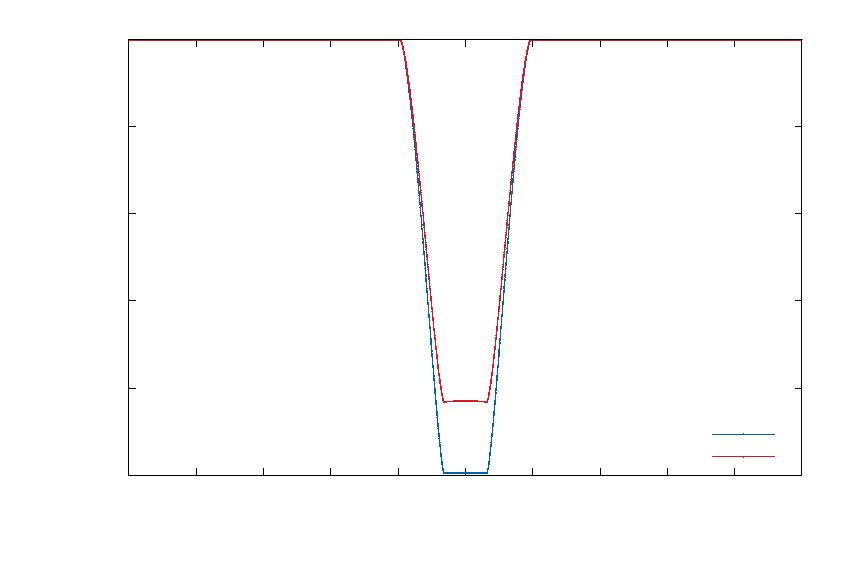
\includegraphics[width={396.80bp},height={255.10bp}]{figures/ellipse-circle-0.5}}%
    \gplfronttext
  \end{picture}%
\endgroup

  \caption{Ellipsoid and sphere of the same volume ($r_2$ = 1, $a$ = 1.2, $b$ = 0.8333333, $c$ = 1), inclination $i=0.5\pi$ and phase $\alpha_0 = 0$}
\end{figure}
\begin{figure}[H]
  \centering
  % GNUPLOT: LaTeX picture with Postscript
\begingroup
  \makeatletter
  \providecommand\color[2][]{%
    \GenericError{(gnuplot) \space\space\space\@spaces}{%
      Package color not loaded in conjunction with
      terminal option `colourtext'%
    }{See the gnuplot documentation for explanation.%
    }{Either use 'blacktext' in gnuplot or load the package
      color.sty in LaTeX.}%
    \renewcommand\color[2][]{}%
  }%
  \providecommand\includegraphics[2][]{%
    \GenericError{(gnuplot) \space\space\space\@spaces}{%
      Package graphicx or graphics not loaded%
    }{See the gnuplot documentation for explanation.%
    }{The gnuplot epslatex terminal needs graphicx.sty or graphics.sty.}%
    \renewcommand\includegraphics[2][]{}%
  }%
  \providecommand\rotatebox[2]{#2}%
  \@ifundefined{ifGPcolor}{%
    \newif\ifGPcolor
    \GPcolortrue
  }{}%
  \@ifundefined{ifGPblacktext}{%
    \newif\ifGPblacktext
    \GPblacktextfalse
  }{}%
  % define a \g@addto@macro without @ in the name:
  \let\gplgaddtomacro\g@addto@macro
  % define empty templates for all commands taking text:
  \gdef\gplbacktext{}%
  \gdef\gplfronttext{}%
  \makeatother
  \ifGPblacktext
    % no textcolor at all
    \def\colorrgb#1{}%
    \def\colorgray#1{}%
  \else
    % gray or color?
    \ifGPcolor
      \def\colorrgb#1{\color[rgb]{#1}}%
      \def\colorgray#1{\color[gray]{#1}}%
      \expandafter\def\csname LTw\endcsname{\color{white}}%
      \expandafter\def\csname LTb\endcsname{\color{black}}%
      \expandafter\def\csname LTa\endcsname{\color{black}}%
      \expandafter\def\csname LT0\endcsname{\color[rgb]{1,0,0}}%
      \expandafter\def\csname LT1\endcsname{\color[rgb]{0,1,0}}%
      \expandafter\def\csname LT2\endcsname{\color[rgb]{0,0,1}}%
      \expandafter\def\csname LT3\endcsname{\color[rgb]{1,0,1}}%
      \expandafter\def\csname LT4\endcsname{\color[rgb]{0,1,1}}%
      \expandafter\def\csname LT5\endcsname{\color[rgb]{1,1,0}}%
      \expandafter\def\csname LT6\endcsname{\color[rgb]{0,0,0}}%
      \expandafter\def\csname LT7\endcsname{\color[rgb]{1,0.3,0}}%
      \expandafter\def\csname LT8\endcsname{\color[rgb]{0.5,0.5,0.5}}%
    \else
      % gray
      \def\colorrgb#1{\color{black}}%
      \def\colorgray#1{\color[gray]{#1}}%
      \expandafter\def\csname LTw\endcsname{\color{white}}%
      \expandafter\def\csname LTb\endcsname{\color{black}}%
      \expandafter\def\csname LTa\endcsname{\color{black}}%
      \expandafter\def\csname LT0\endcsname{\color{black}}%
      \expandafter\def\csname LT1\endcsname{\color{black}}%
      \expandafter\def\csname LT2\endcsname{\color{black}}%
      \expandafter\def\csname LT3\endcsname{\color{black}}%
      \expandafter\def\csname LT4\endcsname{\color{black}}%
      \expandafter\def\csname LT5\endcsname{\color{black}}%
      \expandafter\def\csname LT6\endcsname{\color{black}}%
      \expandafter\def\csname LT7\endcsname{\color{black}}%
      \expandafter\def\csname LT8\endcsname{\color{black}}%
    \fi
  \fi
    \setlength{\unitlength}{0.0500bp}%
    \ifx\gptboxheight\undefined%
      \newlength{\gptboxheight}%
      \newlength{\gptboxwidth}%
      \newsavebox{\gptboxtext}%
    \fi%
    \setlength{\fboxrule}{0.5pt}%
    \setlength{\fboxsep}{1pt}%
    \definecolor{tbcol}{rgb}{1,1,1}%
\begin{picture}(7936.00,5102.00)%
    \gplgaddtomacro\gplbacktext{%
      \csname LTb\endcsname%%
      \put(946,704){\makebox(0,0)[r]{\strut{}$0.7$}}%
      \put(946,1400){\makebox(0,0)[r]{\strut{}$0.75$}}%
      \put(946,2096){\makebox(0,0)[r]{\strut{}$0.8$}}%
      \put(946,2793){\makebox(0,0)[r]{\strut{}$0.85$}}%
      \put(946,3489){\makebox(0,0)[r]{\strut{}$0.9$}}%
      \put(946,4185){\makebox(0,0)[r]{\strut{}$0.95$}}%
      \put(946,4881){\makebox(0,0)[r]{\strut{}$1$}}%
      \put(1078,484){\makebox(0,0){\strut{}$0$}}%
      \put(1724,484){\makebox(0,0){\strut{}$1000$}}%
      \put(2370,484){\makebox(0,0){\strut{}$2000$}}%
      \put(3016,484){\makebox(0,0){\strut{}$3000$}}%
      \put(3662,484){\makebox(0,0){\strut{}$4000$}}%
      \put(4309,484){\makebox(0,0){\strut{}$5000$}}%
      \put(4955,484){\makebox(0,0){\strut{}$6000$}}%
      \put(5601,484){\makebox(0,0){\strut{}$7000$}}%
      \put(6247,484){\makebox(0,0){\strut{}$8000$}}%
      \put(6893,484){\makebox(0,0){\strut{}$9000$}}%
      \put(7539,484){\makebox(0,0){\strut{}$10000$}}%
    }%
    \gplgaddtomacro\gplfronttext{%
      \csname LTb\endcsname%%
      \put(6552,1097){\makebox(0,0)[r]{\strut{}$\alpha_0 = 0.5\pi$}}%
      \csname LTb\endcsname%%
      \put(6552,877){\makebox(0,0)[r]{\strut{}$\alpha_0 = 0$}}%
      \csname LTb\endcsname%%
      \put(209,2792){\rotatebox{-270.00}{\makebox(0,0){\strut{}brightness}}}%
      \put(4308,154){\makebox(0,0){\strut{}$\frac{1}{20000} t$}}%
    }%
    \gplbacktext
    \put(0,0){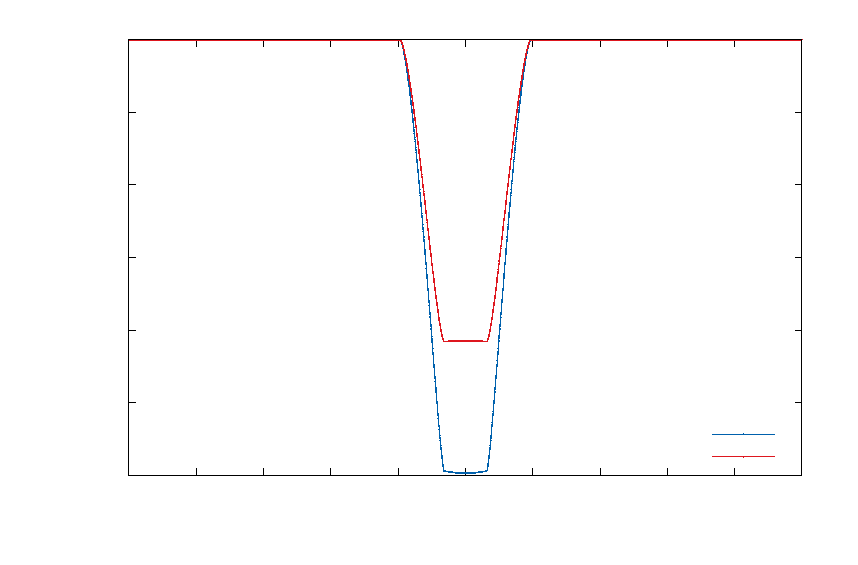
\includegraphics[width={396.80bp},height={255.10bp}]{figures/ellipse-ellipse-different-phase}}%
    \gplfronttext
  \end{picture}%
\endgroup

  \caption{Two ellipsoids with the same $i = 0.5\pi$ and size ($a$ = 1.2, $b$ = 0.8333333, $c$ = 1) but different phase $\alpha_0$}
\end{figure}
\begin{figure}[H]
  \centering
  % GNUPLOT: LaTeX picture with Postscript
\begingroup
  \makeatletter
  \providecommand\color[2][]{%
    \GenericError{(gnuplot) \space\space\space\@spaces}{%
      Package color not loaded in conjunction with
      terminal option `colourtext'%
    }{See the gnuplot documentation for explanation.%
    }{Either use 'blacktext' in gnuplot or load the package
      color.sty in LaTeX.}%
    \renewcommand\color[2][]{}%
  }%
  \providecommand\includegraphics[2][]{%
    \GenericError{(gnuplot) \space\space\space\@spaces}{%
      Package graphicx or graphics not loaded%
    }{See the gnuplot documentation for explanation.%
    }{The gnuplot epslatex terminal needs graphicx.sty or graphics.sty.}%
    \renewcommand\includegraphics[2][]{}%
  }%
  \providecommand\rotatebox[2]{#2}%
  \@ifundefined{ifGPcolor}{%
    \newif\ifGPcolor
    \GPcolortrue
  }{}%
  \@ifundefined{ifGPblacktext}{%
    \newif\ifGPblacktext
    \GPblacktextfalse
  }{}%
  % define a \g@addto@macro without @ in the name:
  \let\gplgaddtomacro\g@addto@macro
  % define empty templates for all commands taking text:
  \gdef\gplbacktext{}%
  \gdef\gplfronttext{}%
  \makeatother
  \ifGPblacktext
    % no textcolor at all
    \def\colorrgb#1{}%
    \def\colorgray#1{}%
  \else
    % gray or color?
    \ifGPcolor
      \def\colorrgb#1{\color[rgb]{#1}}%
      \def\colorgray#1{\color[gray]{#1}}%
      \expandafter\def\csname LTw\endcsname{\color{white}}%
      \expandafter\def\csname LTb\endcsname{\color{black}}%
      \expandafter\def\csname LTa\endcsname{\color{black}}%
      \expandafter\def\csname LT0\endcsname{\color[rgb]{1,0,0}}%
      \expandafter\def\csname LT1\endcsname{\color[rgb]{0,1,0}}%
      \expandafter\def\csname LT2\endcsname{\color[rgb]{0,0,1}}%
      \expandafter\def\csname LT3\endcsname{\color[rgb]{1,0,1}}%
      \expandafter\def\csname LT4\endcsname{\color[rgb]{0,1,1}}%
      \expandafter\def\csname LT5\endcsname{\color[rgb]{1,1,0}}%
      \expandafter\def\csname LT6\endcsname{\color[rgb]{0,0,0}}%
      \expandafter\def\csname LT7\endcsname{\color[rgb]{1,0.3,0}}%
      \expandafter\def\csname LT8\endcsname{\color[rgb]{0.5,0.5,0.5}}%
    \else
      % gray
      \def\colorrgb#1{\color{black}}%
      \def\colorgray#1{\color[gray]{#1}}%
      \expandafter\def\csname LTw\endcsname{\color{white}}%
      \expandafter\def\csname LTb\endcsname{\color{black}}%
      \expandafter\def\csname LTa\endcsname{\color{black}}%
      \expandafter\def\csname LT0\endcsname{\color{black}}%
      \expandafter\def\csname LT1\endcsname{\color{black}}%
      \expandafter\def\csname LT2\endcsname{\color{black}}%
      \expandafter\def\csname LT3\endcsname{\color{black}}%
      \expandafter\def\csname LT4\endcsname{\color{black}}%
      \expandafter\def\csname LT5\endcsname{\color{black}}%
      \expandafter\def\csname LT6\endcsname{\color{black}}%
      \expandafter\def\csname LT7\endcsname{\color{black}}%
      \expandafter\def\csname LT8\endcsname{\color{black}}%
    \fi
  \fi
    \setlength{\unitlength}{0.0500bp}%
    \ifx\gptboxheight\undefined%
      \newlength{\gptboxheight}%
      \newlength{\gptboxwidth}%
      \newsavebox{\gptboxtext}%
    \fi%
    \setlength{\fboxrule}{0.5pt}%
    \setlength{\fboxsep}{1pt}%
    \definecolor{tbcol}{rgb}{1,1,1}%
\begin{picture}(7936.00,5102.00)%
    \gplgaddtomacro\gplbacktext{%
      \csname LTb\endcsname%%
      \put(946,704){\makebox(0,0)[r]{\strut{}$0.7$}}%
      \put(946,1400){\makebox(0,0)[r]{\strut{}$0.75$}}%
      \put(946,2096){\makebox(0,0)[r]{\strut{}$0.8$}}%
      \put(946,2793){\makebox(0,0)[r]{\strut{}$0.85$}}%
      \put(946,3489){\makebox(0,0)[r]{\strut{}$0.9$}}%
      \put(946,4185){\makebox(0,0)[r]{\strut{}$0.95$}}%
      \put(946,4881){\makebox(0,0)[r]{\strut{}$1$}}%
      \put(1078,484){\makebox(0,0){\strut{}$0$}}%
      \put(1724,484){\makebox(0,0){\strut{}$1000$}}%
      \put(2370,484){\makebox(0,0){\strut{}$2000$}}%
      \put(3016,484){\makebox(0,0){\strut{}$3000$}}%
      \put(3662,484){\makebox(0,0){\strut{}$4000$}}%
      \put(4309,484){\makebox(0,0){\strut{}$5000$}}%
      \put(4955,484){\makebox(0,0){\strut{}$6000$}}%
      \put(5601,484){\makebox(0,0){\strut{}$7000$}}%
      \put(6247,484){\makebox(0,0){\strut{}$8000$}}%
      \put(6893,484){\makebox(0,0){\strut{}$9000$}}%
      \put(7539,484){\makebox(0,0){\strut{}$10000$}}%
    }%
    \gplgaddtomacro\gplfronttext{%
      \csname LTb\endcsname%%
      \put(6552,1097){\makebox(0,0)[r]{\strut{}$\alpha_0 = 0.5 \pi$}}%
      \csname LTb\endcsname%%
      \put(6552,877){\makebox(0,0)[r]{\strut{}$\alpha_0 = 0$}}%
      \csname LTb\endcsname%%
      \put(209,2792){\rotatebox{-270.00}{\makebox(0,0){\strut{}brightness}}}%
      \put(4308,154){\makebox(0,0){\strut{}$\frac{1}{20000} t$}}%
    }%
    \gplbacktext
    \put(0,0){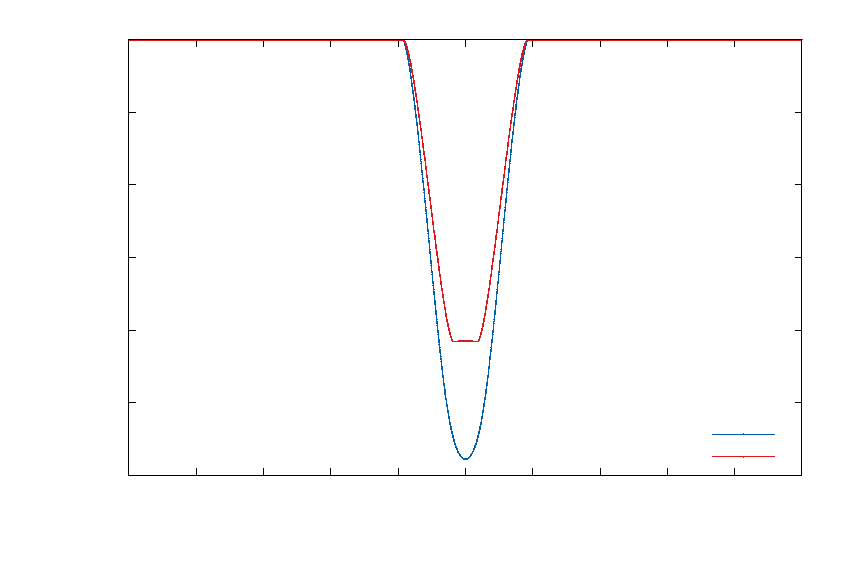
\includegraphics[width={396.80bp},height={255.10bp}]{figures/ellipse-ellipse-0.47-different-phase}}%
    \gplfronttext
  \end{picture}%
\endgroup

  \caption{Two ellipsoids with the same $i = 0.47\pi$ and size ($a$ = 1.2, $b$ = 0.8333333, $c$ = 1), but different phase $\alpha_0$}
\end{figure}
\begin{figure}[H]
  \centering
  % GNUPLOT: LaTeX picture with Postscript
\begingroup
  \makeatletter
  \providecommand\color[2][]{%
    \GenericError{(gnuplot) \space\space\space\@spaces}{%
      Package color not loaded in conjunction with
      terminal option `colourtext'%
    }{See the gnuplot documentation for explanation.%
    }{Either use 'blacktext' in gnuplot or load the package
      color.sty in LaTeX.}%
    \renewcommand\color[2][]{}%
  }%
  \providecommand\includegraphics[2][]{%
    \GenericError{(gnuplot) \space\space\space\@spaces}{%
      Package graphicx or graphics not loaded%
    }{See the gnuplot documentation for explanation.%
    }{The gnuplot epslatex terminal needs graphicx.sty or graphics.sty.}%
    \renewcommand\includegraphics[2][]{}%
  }%
  \providecommand\rotatebox[2]{#2}%
  \@ifundefined{ifGPcolor}{%
    \newif\ifGPcolor
    \GPcolortrue
  }{}%
  \@ifundefined{ifGPblacktext}{%
    \newif\ifGPblacktext
    \GPblacktextfalse
  }{}%
  % define a \g@addto@macro without @ in the name:
  \let\gplgaddtomacro\g@addto@macro
  % define empty templates for all commands taking text:
  \gdef\gplbacktext{}%
  \gdef\gplfronttext{}%
  \makeatother
  \ifGPblacktext
    % no textcolor at all
    \def\colorrgb#1{}%
    \def\colorgray#1{}%
  \else
    % gray or color?
    \ifGPcolor
      \def\colorrgb#1{\color[rgb]{#1}}%
      \def\colorgray#1{\color[gray]{#1}}%
      \expandafter\def\csname LTw\endcsname{\color{white}}%
      \expandafter\def\csname LTb\endcsname{\color{black}}%
      \expandafter\def\csname LTa\endcsname{\color{black}}%
      \expandafter\def\csname LT0\endcsname{\color[rgb]{1,0,0}}%
      \expandafter\def\csname LT1\endcsname{\color[rgb]{0,1,0}}%
      \expandafter\def\csname LT2\endcsname{\color[rgb]{0,0,1}}%
      \expandafter\def\csname LT3\endcsname{\color[rgb]{1,0,1}}%
      \expandafter\def\csname LT4\endcsname{\color[rgb]{0,1,1}}%
      \expandafter\def\csname LT5\endcsname{\color[rgb]{1,1,0}}%
      \expandafter\def\csname LT6\endcsname{\color[rgb]{0,0,0}}%
      \expandafter\def\csname LT7\endcsname{\color[rgb]{1,0.3,0}}%
      \expandafter\def\csname LT8\endcsname{\color[rgb]{0.5,0.5,0.5}}%
    \else
      % gray
      \def\colorrgb#1{\color{black}}%
      \def\colorgray#1{\color[gray]{#1}}%
      \expandafter\def\csname LTw\endcsname{\color{white}}%
      \expandafter\def\csname LTb\endcsname{\color{black}}%
      \expandafter\def\csname LTa\endcsname{\color{black}}%
      \expandafter\def\csname LT0\endcsname{\color{black}}%
      \expandafter\def\csname LT1\endcsname{\color{black}}%
      \expandafter\def\csname LT2\endcsname{\color{black}}%
      \expandafter\def\csname LT3\endcsname{\color{black}}%
      \expandafter\def\csname LT4\endcsname{\color{black}}%
      \expandafter\def\csname LT5\endcsname{\color{black}}%
      \expandafter\def\csname LT6\endcsname{\color{black}}%
      \expandafter\def\csname LT7\endcsname{\color{black}}%
      \expandafter\def\csname LT8\endcsname{\color{black}}%
    \fi
  \fi
    \setlength{\unitlength}{0.0500bp}%
    \ifx\gptboxheight\undefined%
      \newlength{\gptboxheight}%
      \newlength{\gptboxwidth}%
      \newsavebox{\gptboxtext}%
    \fi%
    \setlength{\fboxrule}{0.5pt}%
    \setlength{\fboxsep}{1pt}%
    \definecolor{tbcol}{rgb}{1,1,1}%
\begin{picture}(7936.00,5102.00)%
    \gplgaddtomacro\gplbacktext{%
      \csname LTb\endcsname%%
      \put(946,704){\makebox(0,0)[r]{\strut{}$0.7$}}%
      \put(946,1400){\makebox(0,0)[r]{\strut{}$0.75$}}%
      \put(946,2096){\makebox(0,0)[r]{\strut{}$0.8$}}%
      \put(946,2793){\makebox(0,0)[r]{\strut{}$0.85$}}%
      \put(946,3489){\makebox(0,0)[r]{\strut{}$0.9$}}%
      \put(946,4185){\makebox(0,0)[r]{\strut{}$0.95$}}%
      \put(946,4881){\makebox(0,0)[r]{\strut{}$1$}}%
      \put(1078,484){\makebox(0,0){\strut{}$0$}}%
      \put(1724,484){\makebox(0,0){\strut{}$1000$}}%
      \put(2370,484){\makebox(0,0){\strut{}$2000$}}%
      \put(3016,484){\makebox(0,0){\strut{}$3000$}}%
      \put(3662,484){\makebox(0,0){\strut{}$4000$}}%
      \put(4309,484){\makebox(0,0){\strut{}$5000$}}%
      \put(4955,484){\makebox(0,0){\strut{}$6000$}}%
      \put(5601,484){\makebox(0,0){\strut{}$7000$}}%
      \put(6247,484){\makebox(0,0){\strut{}$8000$}}%
      \put(6893,484){\makebox(0,0){\strut{}$9000$}}%
      \put(7539,484){\makebox(0,0){\strut{}$10000$}}%
    }%
    \gplgaddtomacro\gplfronttext{%
      \csname LTb\endcsname%%
      \put(6552,877){\makebox(0,0)[r]{\strut{}asssymetrical view}}%
      \csname LTb\endcsname%%
      \put(209,2792){\rotatebox{-270.00}{\makebox(0,0){\strut{}brightness}}}%
      \put(4308,154){\makebox(0,0){\strut{}$\frac{1}{20000} t$}}%
    }%
    \gplbacktext
    \put(0,0){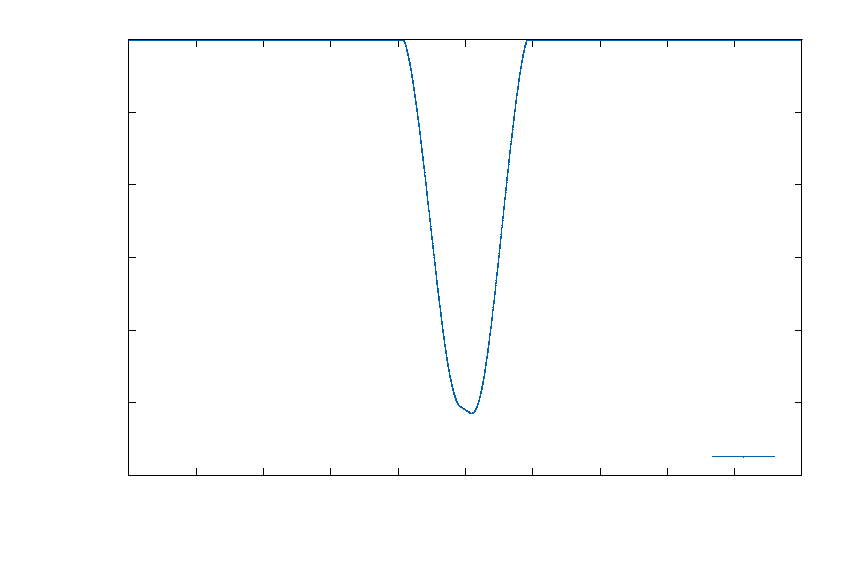
\includegraphics[width={396.80bp},height={255.10bp}]{figures/ellipse-assymetrical}}%
    \gplfronttext
  \end{picture}%
\endgroup

  \caption{Ellipsoid in a more "general" configuration, $a$ = 1.2, $b$ = 0.833333, c = 1, $i$ = 0.47$\pi$, $\alpha_0$ = 0.3$\pi$}
\end{figure}
\begin{figure}[H]
  \centering
  % GNUPLOT: LaTeX picture with Postscript
\begingroup
  \makeatletter
  \providecommand\color[2][]{%
    \GenericError{(gnuplot) \space\space\space\@spaces}{%
      Package color not loaded in conjunction with
      terminal option `colourtext'%
    }{See the gnuplot documentation for explanation.%
    }{Either use 'blacktext' in gnuplot or load the package
      color.sty in LaTeX.}%
    \renewcommand\color[2][]{}%
  }%
  \providecommand\includegraphics[2][]{%
    \GenericError{(gnuplot) \space\space\space\@spaces}{%
      Package graphicx or graphics not loaded%
    }{See the gnuplot documentation for explanation.%
    }{The gnuplot epslatex terminal needs graphicx.sty or graphics.sty.}%
    \renewcommand\includegraphics[2][]{}%
  }%
  \providecommand\rotatebox[2]{#2}%
  \@ifundefined{ifGPcolor}{%
    \newif\ifGPcolor
    \GPcolortrue
  }{}%
  \@ifundefined{ifGPblacktext}{%
    \newif\ifGPblacktext
    \GPblacktextfalse
  }{}%
  % define a \g@addto@macro without @ in the name:
  \let\gplgaddtomacro\g@addto@macro
  % define empty templates for all commands taking text:
  \gdef\gplbacktext{}%
  \gdef\gplfronttext{}%
  \makeatother
  \ifGPblacktext
    % no textcolor at all
    \def\colorrgb#1{}%
    \def\colorgray#1{}%
  \else
    % gray or color?
    \ifGPcolor
      \def\colorrgb#1{\color[rgb]{#1}}%
      \def\colorgray#1{\color[gray]{#1}}%
      \expandafter\def\csname LTw\endcsname{\color{white}}%
      \expandafter\def\csname LTb\endcsname{\color{black}}%
      \expandafter\def\csname LTa\endcsname{\color{black}}%
      \expandafter\def\csname LT0\endcsname{\color[rgb]{1,0,0}}%
      \expandafter\def\csname LT1\endcsname{\color[rgb]{0,1,0}}%
      \expandafter\def\csname LT2\endcsname{\color[rgb]{0,0,1}}%
      \expandafter\def\csname LT3\endcsname{\color[rgb]{1,0,1}}%
      \expandafter\def\csname LT4\endcsname{\color[rgb]{0,1,1}}%
      \expandafter\def\csname LT5\endcsname{\color[rgb]{1,1,0}}%
      \expandafter\def\csname LT6\endcsname{\color[rgb]{0,0,0}}%
      \expandafter\def\csname LT7\endcsname{\color[rgb]{1,0.3,0}}%
      \expandafter\def\csname LT8\endcsname{\color[rgb]{0.5,0.5,0.5}}%
    \else
      % gray
      \def\colorrgb#1{\color{black}}%
      \def\colorgray#1{\color[gray]{#1}}%
      \expandafter\def\csname LTw\endcsname{\color{white}}%
      \expandafter\def\csname LTb\endcsname{\color{black}}%
      \expandafter\def\csname LTa\endcsname{\color{black}}%
      \expandafter\def\csname LT0\endcsname{\color{black}}%
      \expandafter\def\csname LT1\endcsname{\color{black}}%
      \expandafter\def\csname LT2\endcsname{\color{black}}%
      \expandafter\def\csname LT3\endcsname{\color{black}}%
      \expandafter\def\csname LT4\endcsname{\color{black}}%
      \expandafter\def\csname LT5\endcsname{\color{black}}%
      \expandafter\def\csname LT6\endcsname{\color{black}}%
      \expandafter\def\csname LT7\endcsname{\color{black}}%
      \expandafter\def\csname LT8\endcsname{\color{black}}%
    \fi
  \fi
    \setlength{\unitlength}{0.0500bp}%
    \ifx\gptboxheight\undefined%
      \newlength{\gptboxheight}%
      \newlength{\gptboxwidth}%
      \newsavebox{\gptboxtext}%
    \fi%
    \setlength{\fboxrule}{0.5pt}%
    \setlength{\fboxsep}{1pt}%
    \definecolor{tbcol}{rgb}{1,1,1}%
\begin{picture}(7936.00,5102.00)%
    \gplgaddtomacro\gplbacktext{%
      \csname LTb\endcsname%%
      \put(1078,704){\makebox(0,0)[r]{\strut{}$0.975$}}%
      \put(1078,1539){\makebox(0,0)[r]{\strut{}$0.98$}}%
      \put(1078,2375){\makebox(0,0)[r]{\strut{}$0.985$}}%
      \put(1078,3210){\makebox(0,0)[r]{\strut{}$0.99$}}%
      \put(1078,4046){\makebox(0,0)[r]{\strut{}$0.995$}}%
      \put(1078,4881){\makebox(0,0)[r]{\strut{}$1$}}%
      \put(1210,484){\makebox(0,0){\strut{}$0$}}%
      \put(1843,484){\makebox(0,0){\strut{}$5$}}%
      \put(2476,484){\makebox(0,0){\strut{}$10$}}%
      \put(3109,484){\makebox(0,0){\strut{}$15$}}%
      \put(3742,484){\makebox(0,0){\strut{}$20$}}%
      \put(4375,484){\makebox(0,0){\strut{}$25$}}%
      \put(5007,484){\makebox(0,0){\strut{}$30$}}%
      \put(5640,484){\makebox(0,0){\strut{}$35$}}%
      \put(6273,484){\makebox(0,0){\strut{}$40$}}%
      \put(6906,484){\makebox(0,0){\strut{}$45$}}%
      \put(7539,484){\makebox(0,0){\strut{}$50$}}%
    }%
    \gplgaddtomacro\gplfronttext{%
      \csname LTb\endcsname%%
      \put(6552,877){\makebox(0,0)[r]{\strut{}realistic case}}%
      \csname LTb\endcsname%%
      \put(209,2792){\rotatebox{-270.00}{\makebox(0,0){\strut{}relative brightness}}}%
      \put(4374,154){\makebox(0,0){\strut{}time passed $t^{\prime}$ in terms of $\frac{1}{200000}$ $t$ with 25 $t^{\prime}$ being at $\frac{50001}{200000}\ t$}}%
    }%
    \gplbacktext
    \put(0,0){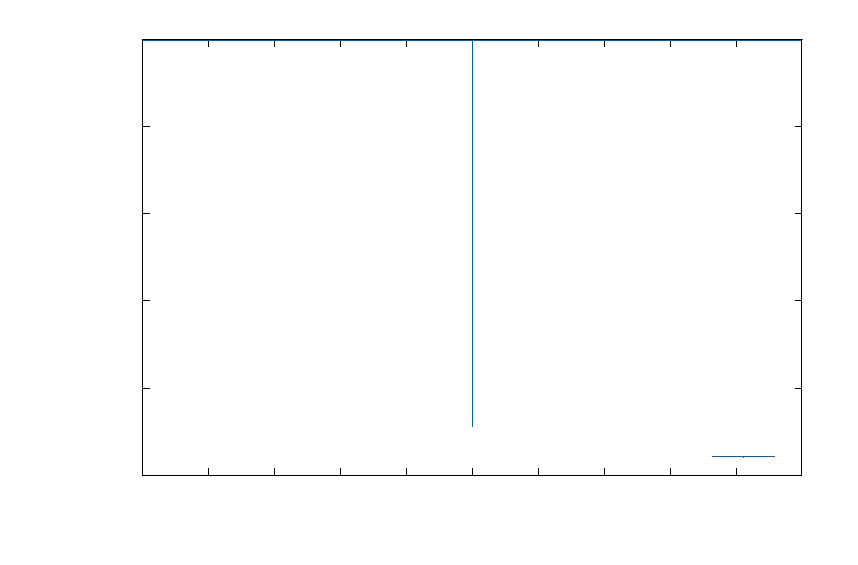
\includegraphics[width={396.80bp},height={255.10bp}]{figures/realistic}}%
    \gplfronttext
  \end{picture}%
\endgroup

  \caption{for the sake of argument, a more "realistic" transit light curve with the parameters:
  $G = 3.0362M_\odot R^3_\odot s^{-2}$, $m_1 = 0.4M_\odot$, $m_2 = 0.002M_\odot$, $r_1 = 0.7R_\odot$, $a = 0.1100R_\odot$, $b = 0.1R_\odot$, $c = 0.1028\odot$, $\alpha_0 = 0.3\pi$, $i = 0.4999\pi$, $r = 1000R_\odot$}
  \label{fig:6}
\end{figure}
\section{Conclusion}
As can be seen above, the transit light curve indeed does depend on the shape of the planet
quite strongly \emph{if the planet is oblate enough}. In our special cases, the planets
were singificantly more oblate than real planets, but as can be seen in figure \ref{fig:6},
detecting any signal at all is difficult enough, moreover, the signal is full of noise
and it becomes increasingly difficult to distinguish a transit from variations in the star's
brightness. In real scenarios, it might be difficult to for example distinguish between
a slightly inclined transit and a transit of an ellipsoidal planet.
\begin{thebibliography}{5}
  \bibitem{carter} Joshua A. Carter and Joshua N. Winn. EMPIRICAL CONSTRAINTS ON THE OBLATENESS OF AN EXOPLANET. 2010 \url{http://dx.doi.org/10.1088/0004-637X/709/2/1219}
  \bibitem{correia1} Alexandre C. M. Correia. Transit light curve and inner structure of close-in planets. 2014. \url{https://doi.org/10.48550/arXiv.0912.1594}
  \bibitem{eeover} Hughes, G.B., Chraibi, M. Calculating ellipse overlap areas. Comput. Visual Sci. 15, 291–301 (2012). \url{https://doi.org/10.1007/s00791-013-0214-3}
\end{thebibliography}
\end{document}
